\documentclass[a4paper,11pt,twoside,openright,article]{memoir}
% Dokumentklassen sættes til memoir.
% Manual: http://ctan.org/tex-archive/macros/latex/contrib/memoir/memman.pdf
\documentclass[a4paper,11pt,twoside,openright,article]{memoir}
\setlrmarginsandblock{*}{2.5cm}{0.75} % højre og venstre 
\setulmarginsandblock{3cm}{*}{1.2} % top og bund 
\checkandfixthelayout[nearest] % specifikt valg af højde algoritme
 
% Danske udtryk (fx figur og tabel) samt dansk orddeling og fonte med
% danske tegn. Hvis LaTeX brokker sig over æ, ø og å skal du udskifte
% "utf8" med "latin1" eller "applemac". 
\usepackage[utf8]{inputenc}
\usepackage[danish]{babel}
\usepackage[T1]{fontenc}
\usepackage{mflogo}

%sexy pdf'er
%\usepackage[export]{adjustbox}
\usepackage{pdfpages}
\usepackage{pdflscape}

%Kompakte lister
\usepackage{paralist}
 
% Matematisk udtryk, fede symboler, theoremer og fancy ting (fx kædebrøker)
\usepackage{amsmath,amssymb}
\usepackage{bm}
\usepackage{amsthm}
\usepackage{mathtools}
\parindent=0pt 

% Fancy ting med enheder og datatabeller. Læs manualen til pakken
% Manual: http://www.ctan.org/tex-archive/macros/latex/contrib/siunitx/siunitx.pdf
\usepackage{siunitx}
 
%Fancy headers, 
%Manual: https://www.sharelatex.com/learn/Headers_and_footers
\let\footruleskip\undefined
\usepackage{fancyhdr}
\pagestyle{fancy}

 
% Indsættelse af grafik. og man kan rotere tekst in line
\usepackage{graphicx} 
\usepackage{fix-cm} 
\usepackage{soul}
\sodef\an{}{0.13em}{0em}{0em} \sodef\ann{}{0.13em}{0.5em}{0em}
 
%Fancy tabeller.
%\usepackage[table]{xcolor}
\usepackage{multirow}
\usepackage{rotating} %sidewaystables!
\usepackage{longtable} %tables spanning multible pages.
\usepackage{tablefootnote} %for at indstætte fornoter i tabeller.
\usepackage{hhline} %Fixer farvede felter
\usepackage{ltxtable} %Longtabular X
\usepackage{tabularx} %Med dynamisk bredte

%URL fodnoter
\usepackage{url}

% Reaktionsskemaer. Læs manualen for at se eksempler.
% Manual: http://www.ctan.org/tex-archive/macros/latex/contrib/mhchem/mhchem.pdf
\usepackage[version=3]{mhchem}

%Lav chapter clickable og fjern border
\usepackage{hyperref}
\hypersetup{
    colorlinks,
    citecolor=black,
    filecolor=black,
    linkcolor=black,
    urlcolor=black
}

%Table of contents settings
\setsecnumdepth{subsection} % organisational level that receives a numbers
\settocdepth{subsection}   % print table of  for level 3

%Til programkode
\usepackage{listings}
\usepackage{color}

\definecolor{dkgreen}{rgb}{0,0.6,0}
\definecolor{gray}{rgb}{0.5,0.5,0.5}
\definecolor{mauve}{rgb}{0.58,0,0.82}
 
\lstset{ 
  language=C++,                % the language of the code
  basicstyle=\footnotesize,           % the size of the fonts that are used for the code
  numbers=left,                   % where to put the line-numbers
  numberstyle=\tiny\color{gray},  % the style that is used for the line-numbers
  stepnumber=1,                   % the step between two line-numbers. If it's 1, each line 
                                  % will be numbered
  numbersep=5pt,                  % how far the line-numbers are from the code
  backgroundcolor=\color{white},      % choose the background color. You must add \usepackage{color}
  showspaces=false,               % show spaces adding particular underscores
  showstringspaces=false,         % underline spaces within strings
  showtabs=false,                 % show tabs within strings adding particular underscores
  frame=single,                   % adds a frame around the code
  rulecolor=\color{black},        % if not set, the frame-color may be changed on line-breaks within not-black text (e.g. commens (green here))
  tabsize=2,                      % sets default tabsize to 2 spaces
  captionpos=b,                   % sets the caption-position to bottom
  breaklines=true,                % sets automatic line breaking
  breakatwhitespace=false,        % sets if automatic breaks should only happen at whitespace
  title=\lstname,                   % show the filename of files included with \lstinputlisting;
                                  % also try caption instead of title
  keywordstyle=\color{blue},          % keyword style
  commentstyle=\color{dkgreen},       % comment style
  stringstyle=\color{mauve},         % string literal style
  escapeinside={\%*}{*)},            % if you want to add LaTeX within your code
  morekeywords={*,...},               % if you want to add more keywords to the set
  rangeprefix=//----------,			%Used for sexy code includes
  rangesuffix=----------,			%---||---
  includerangemarker=false,			%---||---
  literate=
  {á}{{\'a}}1 {é}{{\'e}}1 {í}{{\'i}}1 {ó}{{\'o}}1 {ú}{{\'u}}1
  {Á}{{\'A}}1 {É}{{\'E}}1 {Í}{{\'I}}1 {Ó}{{\'O}}1 {Ú}{{\'U}}1
  {à}{{\`a}}1 {è}{{\`e}}1 {ì}{{\`i}}1 {ò}{{\`o}}1 {ù}{{\`u}}1
  {À}{{\`A}}1 {È}{{\'E}}1 {Ì}{{\`I}}1 {Ò}{{\`O}}1 {Ù}{{\`U}}1
  {ä}{{\"a}}1 {ë}{{\"e}}1 {ï}{{\"i}}1 {ö}{{\"o}}1 {ü}{{\"u}}1
  {Ä}{{\"A}}1 {Ë}{{\"E}}1 {Ï}{{\"I}}1 {Ö}{{\"O}}1 {Ü}{{\"U}}1
  {â}{{\^a}}1 {ê}{{\^e}}1 {î}{{\^i}}1 {ô}{{\^o}}1 {û}{{\^u}}1
  {Â}{{\^A}}1 {Ê}{{\^E}}1 {Î}{{\^I}}1 {Ô}{{\^O}}1 {Û}{{\^U}}1
  {œ}{{\oe}}1 {Œ}{{\OE}}1 {æ}{{\ae}}1 {Æ}{{\AE}}1 {ß}{{\ss}}1
  {ç}{{\c c}}1 {Ç}{{\c C}}1 {ø}{{\o}}1 {å}{{\r a}}1 {Å}{{\r A}}1
  {€}{{\EUR}}1 {£}{{\pounds}}1
}

%Til at udregne forskel mellem sider, brug \pagedifference{A}{B} mellem to labels A og B.
\usepackage{refcount}
\newcommand{\pagedifference}[2]{%
  \number\numexpr\getpagerefnumber{#2}-\getpagerefnumber{#1}\relax}
 
%Til at lave referencer med:
\usepackage{cite}

%Til at lave eksterne \ref til \labels
\usepackage{xr}

%Til at lave \Beam (DC symbol)
\usepackage{marvosym}

%Forsøg på nice lister i tabeller
\usepackage[shortlabels]{enumitem}

\newenvironment{packed_enum}{
\begin{enumerate}[1., topsep=0pt, nosep, partopsep=0pt, itemsep=0pt, parsep=0pt]
}{\end{enumerate}}

\newenvironment{packed_item}{
\begin{itemize}[•, topsep=0pt, nosep, partopsep=0pt, itemsep=0pt, parsep=0pt]
}{\end{itemize}}

%Lækker kommando til at skrive I2C flot uden at bruge \textsuperscript hver gang:
\newcommand*{\IIC}{\texorpdfstring{I\textsuperscript{2}C }{I2C }}

%Lorem ipsum
\usepackage{lipsum}


\usepackage{longtable}
\usepackage{array} % for extrarowheight

%Juicy columntypes - http://tex.stackexchange.com/questions/12703/how-to-create-fixed-width-table-columns-with-text-raggedright-centered-raggedlef
\newcolumntype{L}[1]{>{\raggedright\let\newline\\\arraybackslash\hspace{0pt}}p{#1}}
\newcolumntype{C}[1]{>{\centering\let\newline\\\arraybackslash\hspace{0pt}}p{#1}}
\newcolumntype{R}[1]{>{\raggedleft\let\newline\\\arraybackslash\hspace{0pt}}p{#1}}
\newcolumntype{Z}{>{\raggedright\arraybackslash}X}

%Dejlig kommando til at få nye kapitler på højre side
\newcommand*\cleartorightpage{%
	\clearpage
 	\checkoddpage
	\ifoddpage
  		%do nothing
	\else
		\thispagestyle{empty}
		\mbox{}
 		\clearpage
	\fi
}


%Hacky løsning til at ordne indholdsfortegnelsen.. Why memoir class.. WHY??!
\renewcommand*{\cftdotsep}{1}
\setpnumwidth{3em}
\setrmarg{4em}

%Bugfix til Longtables
\makeatletter
\def\LT@start{%
  \let\LT@start\endgraf
  \endgraf\penalty\z@\vskip\LTpre
  \dimen@\pagetotal
  \advance\dimen@ \ht\ifvoid\LT@firsthead\LT@head\else\LT@firsthead\fi
  \advance\dimen@ \dp\ifvoid\LT@firsthead\LT@head\else\LT@firsthead\fi
  \advance\dimen@ \ht\LT@foot
  \edef\restore@vbadness{\vbadness\the\vbadness\relax}% (added)
  \vbadness=\@M % (added)
  \dimen@ii\vfuzz
  \vfuzz\maxdimen
    \setbox\tw@\copy\z@
    \setbox\tw@\vsplit\tw@ to \ht\@arstrutbox
    \setbox\tw@\vbox{\unvbox\tw@}%
  \vfuzz\dimen@ii
  \restore@vbadness % (added)
  \advance\dimen@ \ht
        \ifdim\ht\@arstrutbox>\ht\tw@\@arstrutbox\else\tw@\fi
  \advance\dimen@\dp
        \ifdim\dp\@arstrutbox>\dp\tw@\@arstrutbox\else\tw@\fi
  \advance\dimen@ -\pagegoal
  \ifdim \dimen@>\z@\vfil\break\fi
      \global\@colroom\@colht
  \ifvoid\LT@foot\else
    \advance\vsize-\ht\LT@foot
    \global\advance\@colroom-\ht\LT@foot
    \dimen@\pagegoal\advance\dimen@-\ht\LT@foot\pagegoal\dimen@
    \maxdepth\z@
  \fi
  \ifvoid\LT@firsthead\copy\LT@head\else\box\LT@firsthead\fi\nobreak
  \output{\LT@output}%
}
\makeatother
%Debugging
%\overfullrule=2cm

\title{Projektrapport \\ Gruppe 1 - AU2 \\ \textit{Den intelligente bil }}
\author{4. Semesterprojekt E4PRJ4 \\ Ingeniørhøjskolen, Aarhus Universitet\\ Vejleder: Arne Justesen}
\date{\today}

%Så man kan hive samtlige \labels i projektdokumentationen, alle har prefix "P-"
\externaldocument[P-]{../projektdokumentation/acceptTest/accepttest}
\externaldocument[P-]{../projektdokumentation/hwdesign/hwdesign}
\externaldocument[P-]{../projektdokumentation/hwimplementering/hwimpl}
\externaldocument[P-]{../projektdokumentation/kravspecifikation/kravspecifikation}
\externaldocument[P-]{../projektdokumentation/litteraturliste/litteraturliste}
\externaldocument[P-]{../projektdokumentation/projektdokumentation/HardwareImplementering}
\externaldocument[P-]{../projektdokumentation/softwareImplementering/swimpl}
\externaldocument[P-]{../projektdokumentation/swdesign/swdesign}
\externaldocument[P-]{../projektdokumentation/systemarkitektur/systemarkitektur}
\externaldocument[P-]{../projektdokumentation/projektformulering/projektformulering}

\begin{document}
\fancyhf{}
\frontmatter
\maketitle
\vfill

\begin{table} [h]
	\centering
	\begin{tabular}{|l|r|l|}
	\hline 
	\textbf{Navn} 				& \textbf{Studienummer} & \textbf{Underskrift~~~~~~~~~~~~~~~~~~~~} 	\\ \hline
	Kristian Thomsen 			& 201311478 & \\ && 												\\ \hline
	Philip Krogh-Pedersen 		& 201311473 & \\ && 												\\ \hline
	Lasse Barner Sivertsen 		& 201371048 & \\ && 												\\ \hline
	Henrik Bagger Jensen 		& 201304157 & \\ && 												\\ \hline
	Kenn Hedegaard Eskildsen 	& 201370904 & \\ && 												\\ \hline
	Karsten Schou Nielsen 		& 201370045 & \\ && 												\\ \hline
	Jesper Pedersen 			& 201370530 & \\ && 												\\ \hline
	\end{tabular}
\end{table}

\clearpage
\pagestyle{plain}

\chapter{Abstract}
\label{ch:Abstract}

This report describes the development of the 4. semester project of engineering bachelor students, in electronic engineering, from Aarhus University of Engineering (ASE).
The project addresses an intelligent car - named AU2 - a remote controlled car, able to be controlled with an Xbox-360 controller\cite{lib:xbox-360} from a common Windows PC.
The intelligent part is based on the car being able to detect a future collision with an obstacle and evading it.
The user is able to monitor the car with a camera\cite{lib:cam} mounted on the car.
The video stream, along with current speed, G-force and distance to nearest obstacle is shown on a program installed on the PC.
A Raspberry Pi 2 B has been applied as controller of the car with a PSoC 4 Pioneer Kit\cite{lib:psoc4_guide} as addon. The PSoC 4 Pioneer Kit utilizes \IIC communication to gather data from the sensors on the car. Amongst the sensors are four proximity sensors\cite{lib:maxsonar}, a homemade tachometer and an accelerometer\cite{lib:accel}.
The software on the Pi has been developed using C++11 threads and a external \IIC library named WiringPi\cite{lib:wiringpi}.
Communication between PC and car is done with Wi-Fi and is implemented through socket based TCP network communication.
The car is driven by a DC-motor, turns with a servomotor and is supplied from a DC-DC buck converter.

The realized system is able to drive the car forward and backward. The user decides the speed through the Xbox-360 controller. The car is able to measure the distance to the nearest obstacle and the current speed. It is able to present the user with the data and video stream on the user interface. The anti-collision system has not been completely implemented. The car is not able to turn because the servomotor have not been installed. Occasional errors have, in addition, been occurring in the communication between the car and the PC.

\clearpage
\chapter{Resume}
\label{ch:Resume}

Denne rapport beskriver udviklingsprocessen for det fjerde semesterprojekt på ingeniørhøjskolen i Århus for elektro linjen. Projektet omhandler en intelligent bil kaldet AU2 som er en legetøjsbil der kan styres fra en almindelig computer med Windows installeret. Den intelligente del består af at bilen selv er i stand til at måle hvornår den er på vej mod en forhindring og derved selv undvige en kollision, på trods af brugerens styreinput. Brugeren er i stand til at se hvor bilen befinder sig via et kamera som er monteret på bilen, samt se bilens aktuelle hastighed mv. i et program installeret på brugerens computer.
\clearpage

\clearpage

\tableofcontents

\vfill

\chapter{Arbejdsopgaver}\label{ch:arbejdsopgaver}
%TODO Ret denne tabel
Under projektarbejdet har arbejdsopgaver været fordelt efter følgende tabel:

\begin{table}[h]
\centering
\begin{tabularx}{\textwidth * 6/7}{Z|l|l|l|l|l|l|l|}
	\cline{2-8}
	~ & \rotatebox{90}{Kristian Thomsen~~} 
	& \rotatebox{90}{Philip Krogh-Pedersen} 
	& \rotatebox{90}{Lasse Barner Sivertsen} 
	& \rotatebox{90}{Henrik Bagger Jensen} 
	& \rotatebox{90}{Kenn Hedegaard Eskildsen} 
	& \rotatebox{90}{Karsten Schou Nielsen} 
	& \rotatebox{90}{Jesper Ellebæk Pedersen}\\ \hline
	\multicolumn{1}{|X|}{Projektformulering} 	& X & X & X & X & X & X & X  \\\hline
	\multicolumn{1}{|X|}{Kravspecifikation} 	& X & X & X & X & X & X & X \\\hline
	\multicolumn{1}{|X|}{Systemarkitektur} 		& X & X & X & X & X & X & X \\\hline
	\multicolumn{1}{|X|}{Protokol GUI} 			&  &  &  &  &  & X &  \\\hline
	\multicolumn{1}{|X|}{Protokol Kamera } 		&  &  &  &  &  & X &  \\\hline
	\multicolumn{1}{|X|}{HW Design og impl. - Bil: Strømforsyning} & X &  &  &  &  &  &  \\\hline
	\multicolumn{1}{|X|}{HW Design og impl. - Bil: Motorstyring} &  &  &  &  &  &  &  X \\\hline
	\multicolumn{1}{|X|}{HW Design og impl. - Bil: Tachometer} &  &  &  &  &  &  & X \\\hline
	\multicolumn{1}{|X|}{SW Design og impl. - Bil: Steering klassen} &  &  &  &  &  &  & X \\\hline
	\multicolumn{1}{|X|}{SW Design og impl. - PC: Software} &  &  &  &  &  & X &  \\\hline
	\multicolumn{1}{|X|}{SW Design og impl. - PC: XboxController klassen} &  &  & X &  &  &  &  \\\hline
	\multicolumn{1}{|X|}{SW Design og impl. - Bil: Kamera software} &  &  &  &  &  & X &  \\\hline
	\multicolumn{1}{|X|}{SW Design og impl. - Bil: Log og Data klasserne} &  & X &  &  &  &  &  \\\hline
	\multicolumn{1}{|X|}{SW Design og impl. - Bil: PcCom og Settings klasserne} &  &  & X &  &  &  &  \\\hline
	\multicolumn{1}{|X|}{SW Design og impl. - Bil: DistanceSensor} &  &  &  &  & X &  &  \\\hline
	\multicolumn{1}{|X|}{SW Design og impl. - Bil: Aks og Pi klasserne} & X &  &  &  &  &  &  \\\hline
	\multicolumn{1}{|X|}{Accepttest} & X & X & X & X & X & X & X  \\\hline
	\multicolumn{1}{|X|}{Rapport} & X & X & X & X & X & X & X \\\hline
	\end{tabularx}
\end{table}

\mainmatter

\pagestyle{fancy}
\fancyhf{} %Clear all header/footers
\fancyhead[RO,LE]{Gruppe 1 - AU2}
\fancyhead[CE,CO]{\nouppercase{\leftmark}}
\fancyhead[LO,RE]{IHA, AU}
\fancyfoot[CO,CE]{\nouppercase{\rightmark}}
\fancyfoot[LE,RO]{\thepage}

\chapter{Forord}
\label{ch:Forord}

%TODO
Projektgruppen er bestående af i alt 7 mand og alle har bidraget til systemarkitekturen samt deltaget aktivt i oprettelsen af usecasene i aktitekturfasen. Det meste i designfasen blev også lavet af hele gruppen men i implementeringen blev det delt op i mindre grupper eller enkelte personer. Rapporten indeholder derfor sektioner som er skrevet samlet, samt individuelle sektioner. De individuelle sektioner er skrevet ud fra personernes ansvarsområde i implementeringsfasen. Disse ses under Arbejdsopgaver.  

\clearpage
\chapter{Indledning}
\label{ch:Indledning}

Denne rapport indeholder beskrivelsen af udvikling og design for 4. semesterprojektet, AU2, samt opbygningen af en prototype. 
Rapporten er opsummeringen af projektdokumentationen, og dækker hovedsageligt over udviklingsmæssige overvejelser/beslutninger som gruppen har foretaget undervejs i projektperioden. 
Bilen gør det muligt for børn og voksne at underholdes uden risiko for at ødelægge bilen, eftersom den selv forhindrer en forestående kollision.

AU2 er en intelligent bil, som vha. et antikollisions system (AKS) kan undvige en detekteret forhindring, og desuden styres med en X-Box Controller over et trådløst Wi-Fi netværk. Bilen kan bremse, dreje, køre frem og tilbage.
I forbindelse med en nærtstående kollision, vil AKS overtage styringen fra brugeren, og dreje bilen i en anden mindre farlig retning. 
Projektet består af en PC med tilhørende X-Box Controller, en Raspberry Pi med tilhørende Wi-Fi Dongle og en PSoC. 

Brugeren kan se hvor bilen kører vha. det påmonterede kamera, hvorfor det er muligt at styre bilen fra et punkt hvor bilen ikke er synlig.
GUI på PC er lavet i QT og brugeren ser data om bilen i sammnhæng med videoen, der streames fra bilen.

\section{Læsevejledning}
Projektdokumentationen til denne rapport er skrevet kronologisk i forhold til de givne faser i ASE Modellen\cite{lib:vejledning}, pånær accepttesten, som er udarbejdet i forlængelse af kravspecifikationen, men selve testen er udført i slutningen af forløbet, deraf placeringen sidst i dokumentet.
Den samme rækkefølge er ført i denne rapport under kapitel \ref{ch:Projektbeskrivelse} \nameref{ch:Projektbeskrivelse}.

Da projektet er blevet delt op i enkelte ansvarsområder efter fuldendt systemarkitektur, indeholder rapporten samt dokumentationen både afsnit skrevet at den samlede gruppe samt individuelle afsnit.
Bemærk at der på side '\pageref{ch:arbejdsopgaver}' er vist en tabel med arbejdsopgaver, som beskriver hvad de enkelte gruppemedlemmers ansvarsområder har været i projektet. 
Dette betyder dog ikke at det nødvendigvis kun er markerede personer der har skrevet i de givne afsnit i rapporten, men at disse personer er ansvarlige for den del af projektet i sin helhed.
I starten af hvert kapitel i projektdokumentationen, er der tilknyttet en versionshistorik, som har påført initialer for hvem der har indført materialet, ikke nødvendigvis hvem der har lavet det.

\clearpage

\section{Ordforklaring}

\begin{table}[h]
\centering
\begin{tabularx}{\textwidth*9/10}{| l | Z |}
% header ------------------------
\hline
\textbf{Begreb} & \textbf{Forklaring} \\\hline
% header ------------------------
	At lave noget fornuftigt & 
	Sidde på en stol med en kop kaffe og stirre ud af vinduet. \\\hline
	Skænderi &
Når kaffekanden er tom \\\hline
	Systemlog &
Systemet er udstyret med en log over hvad systemet foretager sig. Dette kunne f.eks. være et indlæg når systemet foretager en måling, sender en e-mail og regulerer miljøet i drivhuset. \\\hline
	Virtuelt Drivhus &
Det virtuelle drivhus er systemets repræsentation af det fysiske drivhus. Brugeren kan tilføje planter fra plantedatabasen i det virtuelle drivhus, og på den måde give systemet indirekte oplysninger om ønskede parametre. Disse informationer lagres i systemets konfigurationsfil. \\\hline
	Fysisk Drivhus &
Ved det fysiske drivhus forstås det drivhus, hvori systemet er monteret. \\\hline
	Konfigurationsfil &
Dette er en klasse, der er placeret på DevKit8000, som indeholder brugerens konfigurationer om blandt andet notifikationer, e-mailadresser, antallet af fugtsensorer og deres unikke ID mm. \\\hline
	Notifikations e-mail &
Dette er en daglig e-mail, som brugeren kan vælge at få tilsendt. Den sendes klokken 12:00, og indeholder informationer om parametrene i det fysiske drivhus. \\\hline
	Advarsels e-mail &
Dette er en e-mail, som brugeren kan vælge at få tilsendt. Den sendes, hvis en parameter i det fysiske drivhus kommer uden for tolerancen af den ønskede værdi. \\\hline
\end{tabularx}
\end{table}
%TODO lave ordforklaring
\clearpage
\chapter{Opgaveformulering}
\label{ch:Opgaveformulering}

%TODO Er dette afsnit redundant? /KT

OBS: Stjålet fra PRJ3

Herunder er vist en prioritering af funktionaliteter i systemet efter MoSCoW metoden. 

Ambitionen for dette projekt var som absolut minimum, at realisere nedenstående punkter under \textit{"skal"}. 
Det forventedes desuden at punkterne under \textit{"bør"} skulle realiseres, men de har haft lavere prioritet.
Punkterne under \textit{"kan"} forventedes ikke realiseret, og punkterne under \textit{"vil ikke..."} realiseredes med sikkerhed ikke. 
Sidstnævnte punkter kan ses som udviklingsmuligheder i forhold til senere versioner af systemet. 

\begin{itemize}
	\item \textbf{Systemet skal:}
		\begin{itemize}
			\item Kunne monitorere temperaturen i drivhuset og regulere temperaturen i drivhuset vha. varmelegeme, åbning af vinduer og luftcirkulation.
			\item Give brugeren mulighed for at vælge varmelegeme og/eller luftcirkulation fra, hvis en mere økonomisk regulering af temperaturen ønskes. 
			\item Have et grafisk user interface.
		\end{itemize}
	\item \textbf{Systemet bør:}
		\begin{itemize}
			\item Måle jordfugtighed med op til seks sensorer i drivhuset og give brugeren besked på brugerfladen om, at det er tid til at vande. 
			\item Måle lysintensitet og luftfugtighed i drivhuset.
			\item Indeholde en log over alle målte parametre: Jordfugtighed, temperatur, luftfugtighed og lysintensitet. 
			Dataene præsenteres grafisk for brugeren.
			\item Indeholde en database over de mest almindelige drivhusplanter, så brugeren kan orientere sig om en plantes optimale forhold.
			\item Indeholde en systemlog, som noterer vigtige system hændelser.
		\end{itemize}
	\item \textbf{Systemet kan:}
		\begin{itemize}
			\item Sende besked til brugeren via e-mail, om at det er tid til at vande.
			\item Tilkobles et automatisk vandingssystem, som aktiveres ved behov for vanding. 
			\item Give brugeren mulighed for at tilføje planter i databasen.
			\item Give brugeren mulighed for at kommunikere trådløst med systemet fra brugerfladen, så denne kan placeres fx inde i brugerens bolig. 
		\end{itemize}
	\item \textbf{Systemet vil ikke i denne version:}	
		\begin{itemize}
			\item Indeholde et kamera, og tilhørende billedarkiv, som giver brugeren mulighed for at følge planternes udvikling fra dag til dag. 
			\item Give brugeren mulighed for at interagere med systemet via en app på dennes mobiltelefon. 
		\end{itemize}
\end{itemize}

For den fulde tekst se afsnit \ref{P-ch:projektformulering} \nameref{P-ch:projektformulering} på side \pageref{P-ch:projektformulering} i projektdokumentationen.

\clearpage
\chapter{Projektafgrænsning} \label{ch:Projektafgraensning}

Systemet AU2 er bygget på en skrabet fjernstyret bil, hvor kun chassiset, hjulene og DC-motoren er tilbage. På denne platform er der tilføjet en Raspberry Pi 2 B med kamara og Wi-Fi dongle, et PSoC 4 Pioneer kit, en strømforsyning med batteri, et tachometer-modul, fire afstandssensorer, et accelerometer, et motorstyrings-modul inkl. servomotor. Den anden side af projektet omfatter den software der er på PCen og den tilsluttede Xbox-360 controller. Selv PCen og Wi-Fi netværket er ikke en del af systemet, men skal være tilgængeligt for at systemet kan fungere. En mere detaljeret beskrivelse af bilens opdeling i blokke kan findes i afsnit \ref{P-sec:BDD_for_AU2} \nameref{P-sec:BDD_for_AU2} på side \pageref{P-sec:BDD_for_AU2} i dokumentationen.\\\\


%TODO
\textbf{OBS: Stjålet fra PRJ3}

AutoGreen består af en strømforsyning, en række controllere (tre stk. PSoC 4 Pioneer Kits og et stk. DevKit8000), et varmelegeme (en USB strømspareskinne og en 100W 230V AC glødepære), fire 12V DC ventilatorer og en 12V steppermotor - samt tilhørende mosfet drivere. 
AutoGreen uindeholder desuden sensorer til måling af lufttemperatur, jordfugt, lysintensitet og luftfugtighed.

Selve det fysiske drivhus er således ikke en del af systemet. 
Under udviklingen af denne prototype er anvendt en model af et drivhus på ca. 33 liter, se evt. Figur \ref{P-fig:dimensioner} på side \pageref{P-fig:dimensioner} i Projektdokumenationen. 
Såfremt prototypen skal monteres i et rigtigt drivhus, skal ventilatorer og varmelegeme dimensioneres derefter.

\mbox{}

I de indledende faser af projektarbejdet - Projektformulering, Kravspecifikation, Accepttestspecifikation og Systemarkitektur - omhandler projektdokumentationen det fulde system.
Grundet tidsnød og forskellige komplikationer, er der flere dele af det samlede system, som kun er delvist eller slet ikke implementeret.
Prioriteringen af hvad der skulle skæres væk undervejs har taget udgangspunkt i MoSCoW prioriteringen, se afsnit \ref{ch:Opgaveformulering} \nameref{ch:Opgaveformulering} på side \pageref{ch:Opgaveformulering}.

Alle punkter under "Systemet skal"\ er fuldt implementeret. 

Under "Systemet bør"\ er det første punkt, vedrørende jordfugtsensorer, fuldt implementeret; øvrige punkter er kun delvist eller slet ikke implementeret.

Punkter under "Systemet kan"\ og "Systemet vil ikke i denne version"\ er ikke implementeret. 

Det er med fuldt overlæg at denne løbende prioritering har fundet sted. 
Gruppen ønskede fra starten et system med mange muligheder for udvikling og udbygning; derfor blev der fra begyndelsen beskrevet et system, som var væsentligt mere omfattende, end hvad gruppen regnede med at kunne nå at realisere.

\mbox{}

Den gennemførte acceptest (af hele det beskrevne system) giver detaljeret information om hvad der er realiseret, hvad der er delvist realiseret og hvad der ikke er realiseret, se afsnit \ref{P-ch:Accepttest} \nameref{P-ch:Accepttest} på side \pageref{P-ch:Accepttest} i projektdokumentationen. 


\clearpage
\chapter{Systembeskrivelse} \label{ch:Systembeskrivelse}
Systemet består samlet af en PC, en Xbox-360 controller og en legetøjsbil som styres fra PC'en. Legetøjsbilen styres via et netværk som kræver at både PC og bil er logget på samme router. Bilen tilkobles en trådløs forbindelse hvorimod PC sagtens kan tilgå netværket via kabel. I projektet er der blevet designet en GUI som køres på PC'en således brugeren er i stand til at modtage et video-stream fra bilen. På den måde er brugeren i stand til at styre bilen uden at kunne se den fysisk. På bilen er påmonteret sensor således brugeren er i stand til at aflæse bilens hastighed, acceleration og afstand til forhindring. Den intelli

\chapter{Krav}\label{ch:Krav} %Please start me on a left page :)

I dette afsnit er de opstillede krav for AU2 beskrevet.
Disse krav er opstillet ud fra opgaveformuleringen og ud fra forestillinger om relevante test af systemet. 
Funktionelle krav er opstillet ud fra Use Cases og ikke-funktionelle krav er opstillet ud fra relevante målbare størrelser.

I figur \ref{fig:use_cases} på side \pageref{fig:use_cases} ses Use Cases for systemet samt en kort beskrivelse af dem. 
De funktionelle krav for systemet er udledt ud fra disse og beskrevet herunder. 
For at se den komplette beskrivelse af kravene for systemet henvises til kapitel \ref{P-ch:kravspecifikation} \nameref{P-ch:kravspecifikation} på side \pageref{P-ch:kravspecifikation} i dokumentationen.

\begin{itemize}
%\begin{packed_item}

\item \textbf{UC1: Aktiver system} sørger for at initialisere systemet ved opstart og beskriver brugerens interaktion med systemet ved opstart.

\item \textbf{UC2: Stream video} initialiserer og vedligeholder streaming af video og beskriver hvad brugeren ser når systemets videostream startes.

\item \textbf{UC3: Overvåg sensorer} indsamler data fra bilens sensorer og analyserer om en undvigelsesmanøvre er nødvendig for at bilen ikke kører ind i noget.

\item \textbf{UC4: Undvig forhindring} styrer automatisk bilen udenom en forhindring ved at manipulere bilens styrtøj og motor.

\item \textbf{UC5: Kør bil frem/tilbage} beskriver brugerens interaktion med systemet når vedkommende ønsker at køre fremad eller at bakke. 
Det beskrives ligeledes hvordan AKS overtager kontrol over bilen for at undvige forhindringer.

\item \textbf{UC6: Drej bil til højre/venstre} beskriver brugerens interaktion med systemet når brugeren ønsker at få bilen til at dreje til enten højre eller venstre. Beskriver ydermere AKS' overtagelse af kontrollen af bilen.

\item \textbf{UC7: Brems bil} beskriver hvordan bilen bremses både af bruger og af AKS.

\item \textbf{UC8: Konfigurer IP-adresse} beskriver hvordan brugeren indstiller IP-adressen for bilen i PC softwaren

\item \textbf{UC9: Tænd/sluk AKS} beskriver hvordan brugeren slår AKS fra eller til.

\item \textbf{UC10: Indstil makshastighed} beskriver hvordan brugeren indstiller en ny makshastighed for bilen.

\item \textbf{UC11: Kalibrer styrtøj} beskriver hvordan brugeren kalibrer styrtøjet, så bilen kører ligeud.

\item \textbf{UC12: Afbryd system} beskriver hvad der sker, når systemet afbrydes eller lukkes ned af brugeren.

%\end{packed_item}
\end{itemize}

De funktionelle krav til systemet er opstillet som følge. Bilen skal kunne køre frem og tilbage, dreje og give brugeren mulighed for at begrænse makshastigheden af bilen. 
Styringen af bilen skal foregå med en Xbox-360 Controller fra en PC via et Wi-Fi netværk til bilens Raspberry Pi.
Bilen skal selv via afstandssensorerne kunne identificere en forhindring i bilens køreretning, og hvis AKS er aktiveret skal dette styre bilen udenom forhindringen eller bremse bilen.
Brugeren skal ydermere via den grafiske brugerflade på PC'en kunne se et live video feed fra et kamera ombord på bilen.
Brugeren bør kunne aktivere og deaktivere AKS ved hjælp af PC softwaren.
Bilen bør være udstyret med bremselys, som lyser ved bremsning.

De ikke-funktionelle krav findes i afsnit \ref{P-sec:ikke-funktionelle_krav} \nameref{P-sec:ikke-funktionelle_krav} på side \pageref{P-sec:ikke-funktionelle_krav} i dokumentationen.

\clearpage

\begin{figure}[h]
\centering
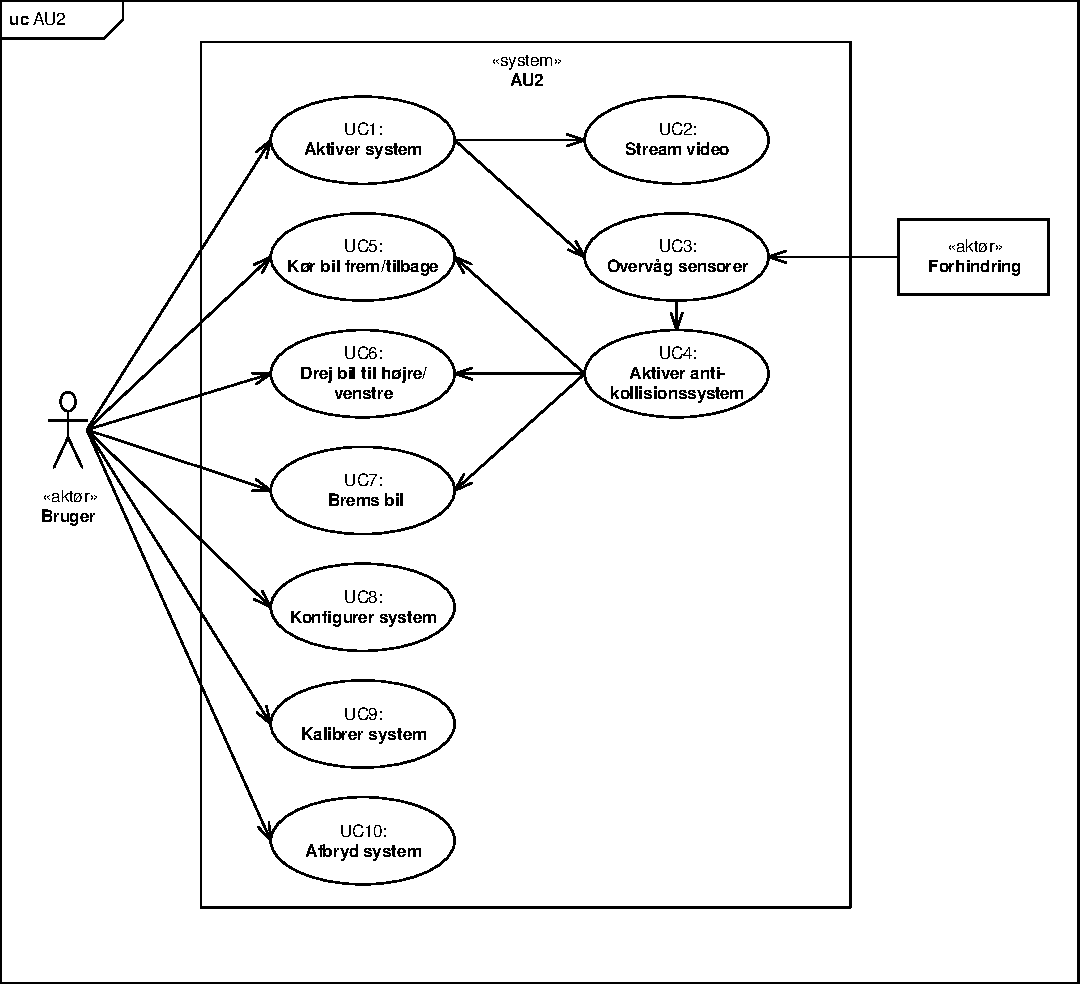
\includegraphics[width=\textwidth]{../fig/diagrammer/uc_au2}
\caption{Use Cases for AU2.}
\label{fig:use_cases}
\end{figure}
\chapter{Projektbeskrivelse}

Svissen svassen

\chapter{Konklusion}
\label{ch:Konklusion}

Jf. kapitel \myRef{P-ch:Accepttest} i dokumentationen ses det, at der fortsat er arbejde at udføre henimod udgivelse af en færdig prototype.
Projektet har været meget lærerigt og gruppen har oplevet en stor succes med sammensætning af de forskellige moduler af projektet. 
Kernen i denne arbejdsgang er at hver enkelt gruppemedlems arbejde har medvirket til en stor fremdrift for projektet. 
Kommunikationsvejene fra bruger til sensor er implementeret, men giver dog sporadiske udfald. 
De væsentligste ting på projektet er implementeret og fungerer som forventet, dog mangler der enkelte steder at blive finjusteret og fejlsøgt. 

Gennem samarbejde og et gennemgående engagement, har gruppen formået at planlægge et realistisk projekt fra start og endt ud med en fungerende prototype. 
Der er løbende i projektfasen opstået flere udfordringer, som har ledt til  designændringer undervejs. 
Flere af de ikke-beståede punkter i accepttesten, er ikke godkendt pga. manglende implementering. 
For de udeladte elementer i projektet er der foretaget undersøgelser og forberedelser til at kunne implementere disse evt. som del af fremtidig arbejde. 
Blandt de elementer der mangler at blive implementeret er bla. accelerometeret, servomotor, fuld AKS-funktionalitet samt motorprint. 
Disse er enten skåret fra projektet, eller udeladt af hensyn til tidsplanen. 
Gruppen har fra projektstart været enige om at det er bedre at skære noget fra projektet i sidste ende, end at begrænse projektet for meget. 
Dog erkendes det at valget at skære de nævnte elementer fra er sket for sent, ift. hvad der havde været optimalt for projektet.

Blandt fremtidigt arbejde er de største udviklingspotentialer i servomotoren, motorprintet og AKS-klassen, således bilen får mulighed for at dreje og rent faktisk undvige en forhindring. 
Der kan læses mere om udfordringerne med disse moduler hhv. i afsnit \myRef{P-sec:hwi_servo}, \myRef{P-sec:hwi_motor_driver} og \myRef{P-sec:aks_impl} i dokumentationen. 

Projektgruppen er en kombination af to forskellige grupper der hver især har haft deres arbejdsmetoder.
En vigtig del af projektet har været at  tilpasse arbejdsmetoderne bedst muligt, og hermed opnå et optimalt samarbejde hvor der kunne trækkes på andres erfaringer. 
I forbindelse med dette har der været en naturlig indkøringsperiode for den nydannede gruppe.

Forløbet har resulteret i en gruppe som nu er stærkt bundet sammen i et samarbejde, som har formået at løfte hele projektet og gjort det muligt at komme så langt. 
Gruppen har været i konstant udvikling både fagligt og socialt og alle har fået rykket deres kompetencer indenfor gruppearbejde endnu en gang.

Tidsplanen er blevet holdt nogenlunde fast, med undtagelse af implementerings og testperioden, som gik lidt over planlagt tid. 
Til sidst kan gruppen konkludere at E4PRJ4 har været et udfordrende og lærerigt projekt såvel fagligt som socialt.

\clearpage
\include{Litteraturliste/Litteraturliste}

\clearpage
~ 

\end{document}
